\section*{Motivation}

\begin{frame}{Social-Network Analysis}
    \begin{figure}[h]
        \centering
        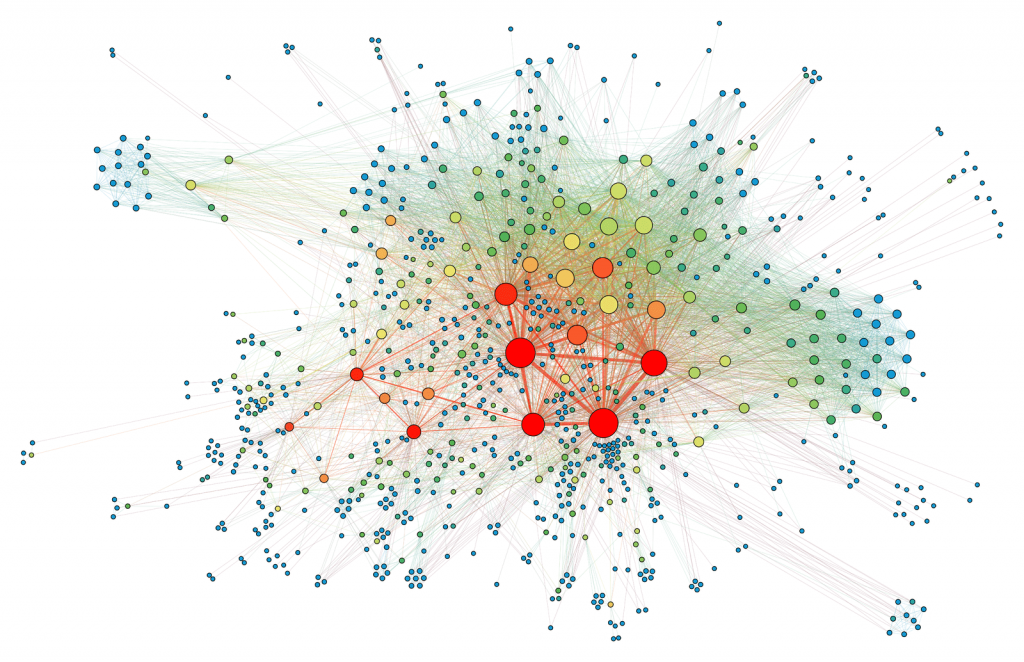
\includegraphics[width=0.65\textwidth]{imglib/social-network-analysis}\\
        \label{fig:social-network-analysis}
    \end{figure}
\end{frame}

\begin{frame}{Social-Network Analysis}
    \begin{itemize}
        \item Wer kennt wen?
        \item Wer kennt wen, den ich kenne?
        \item Wer kennt viele, die sich untereinander auch kennen?
        \item Gibt es Gruppen, in denen (fast) jeder jeden kennt?
        \item Wie finde ich besonders eng verbundene Gemeinschaften?
        \item Wie stabil oder robust sind diese Gruppen gegen den Verlust von Verbindungen?
    \end{itemize}
\end{frame}

\begin{frame}{Higher-Order Truss-Decomposition}
    \begin{itemize}
        \item \textbf{Decomposition}: Zerlegung
        \item \textbf{Truss}: Gerüst
        \item \textbf{To truss something}: etwas bündeln
        \item \textbf{Higher-Order}: höherer Ordnung
    \end{itemize}
\end{frame}
